\chapter{Representation of vortex variability in climate models}
\label{cha:models}


\begin{figure}
 \centering
 \noindent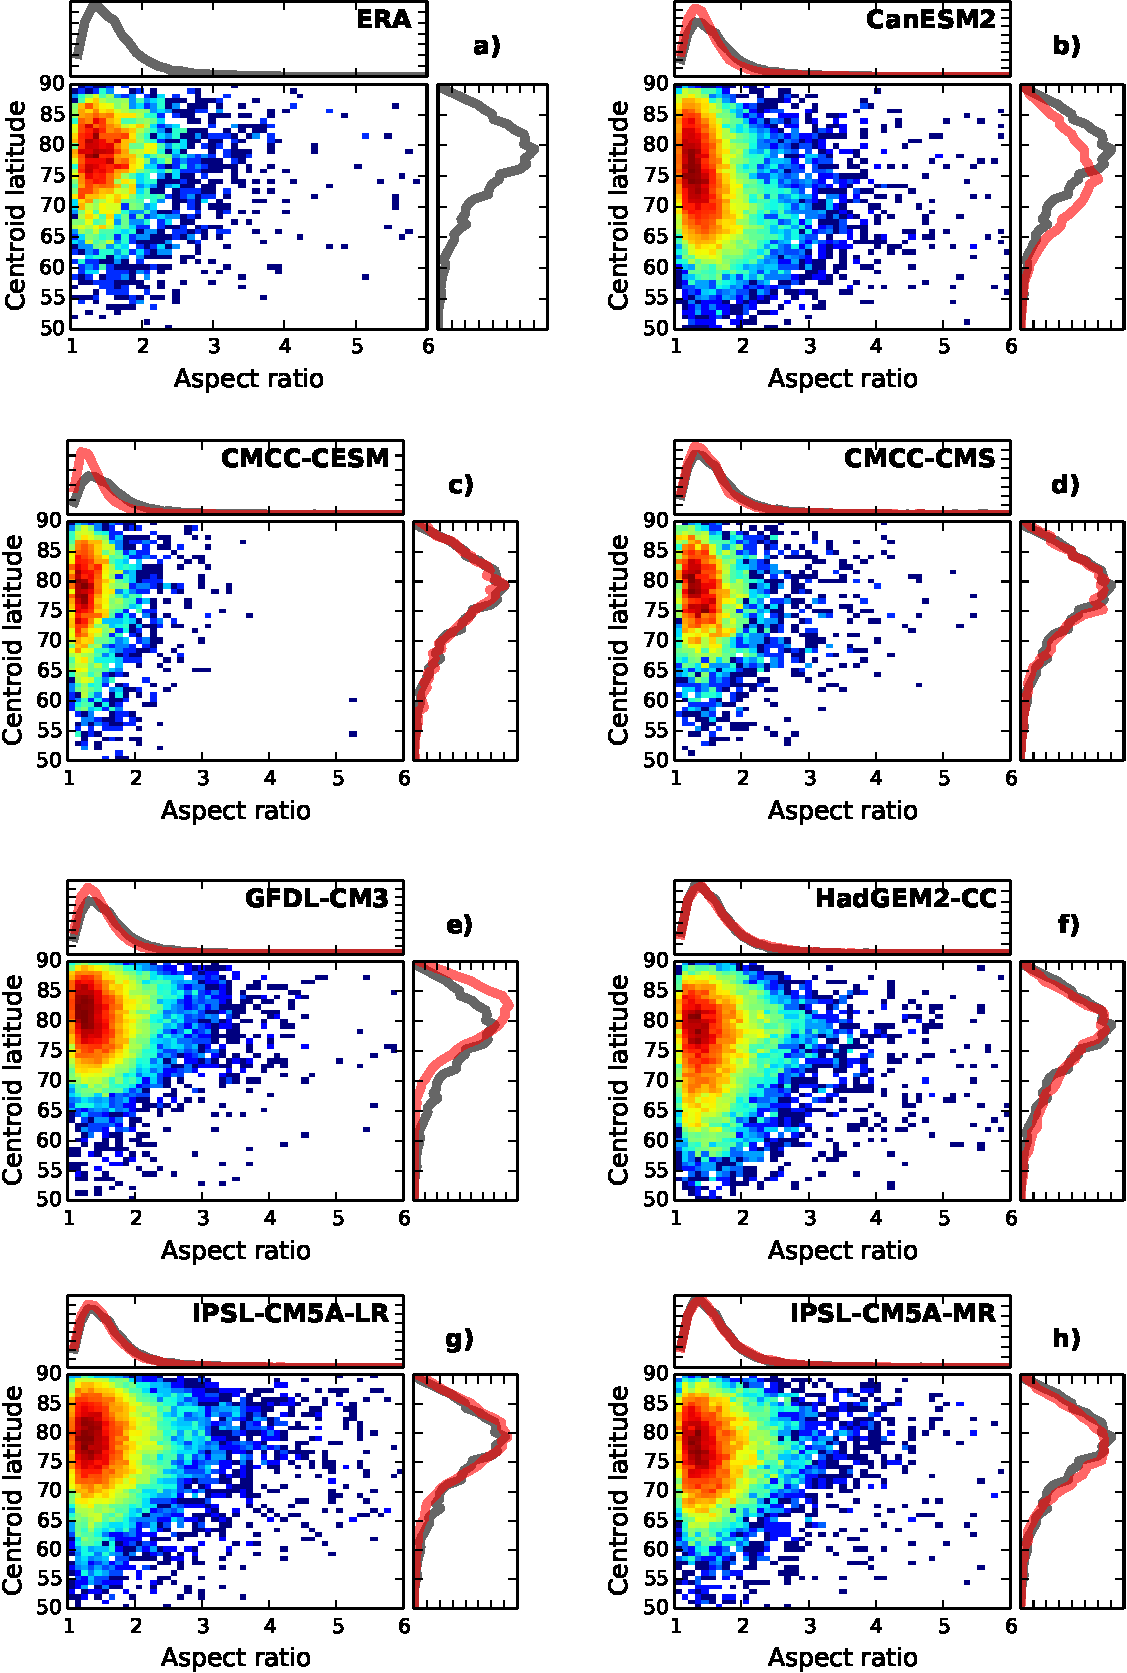
\includegraphics[width=\textwidth]{figures/chapter-models/moments_stats1.pdf}
 \caption[Distributions of moment diagnostics for the CMIP5
 models.]{Distributions of centroid latitude and aspect ratio for the ERA (grey
   lines) (a) and the CMIP5 models (red lines). Joint distributions are shown
   with a logarithmic scale such that red squares represent the densest
   regions.}
 \label{Fig2}
\end{figure}

\begin{figure}
 \ContinuedFloat
 \centering
 \noindent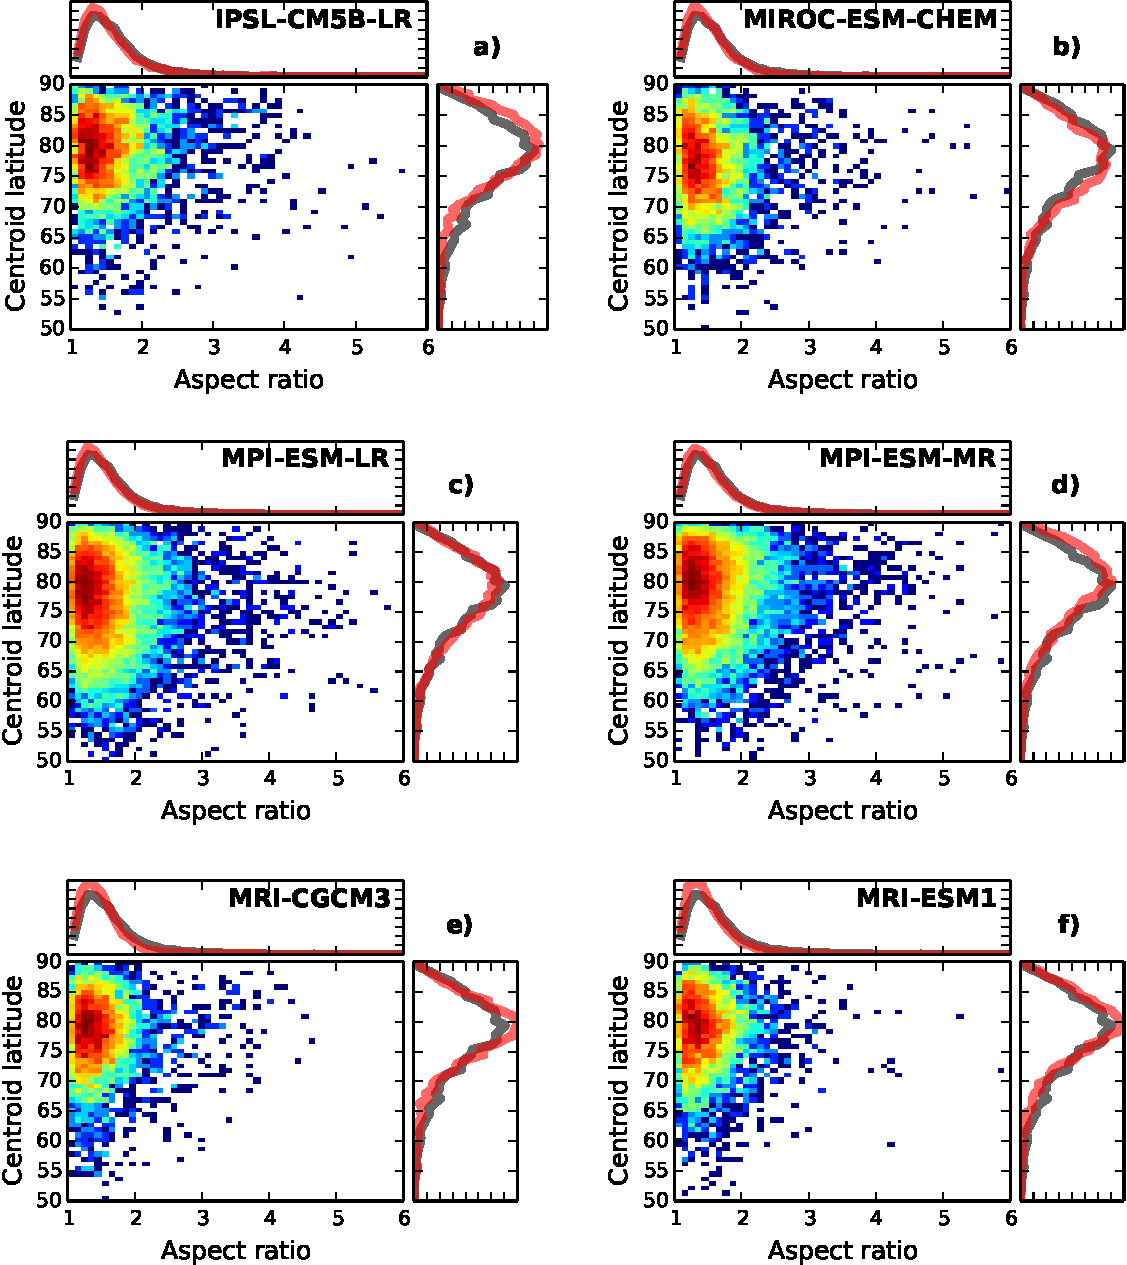
\includegraphics[width=\textwidth]{figures/chapter-models/moments_stats2.pdf}
 \caption[]{(Continued)}
 \label{Fig2}
\end{figure}
 
\begin{figure}
 \centering
 \noindent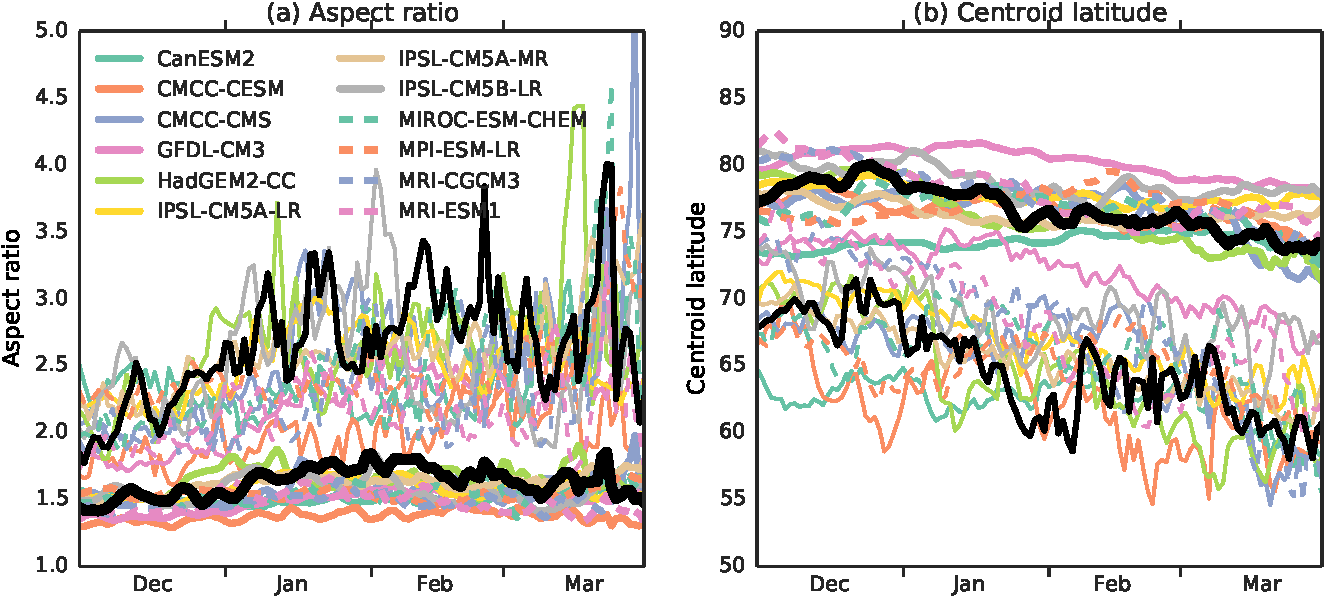
\includegraphics[width=\textwidth]{figures/chapter-models/moments_seasonal_stats.pdf}
 \caption[Seasonal cycle of moment diagnostics in the CMIP5 models]{Seasonal
   cycle of aspect ratio and centroid latitude in ERA (black) and the CMIP5
   models (colours). Thick lines represent the mean and thin lines the 95th or
   5th percentile for aspect ratio and centroid latitude respectively.}
 \label{Fig2}
\end{figure}



\begin{figure}
 \centering
 \noindent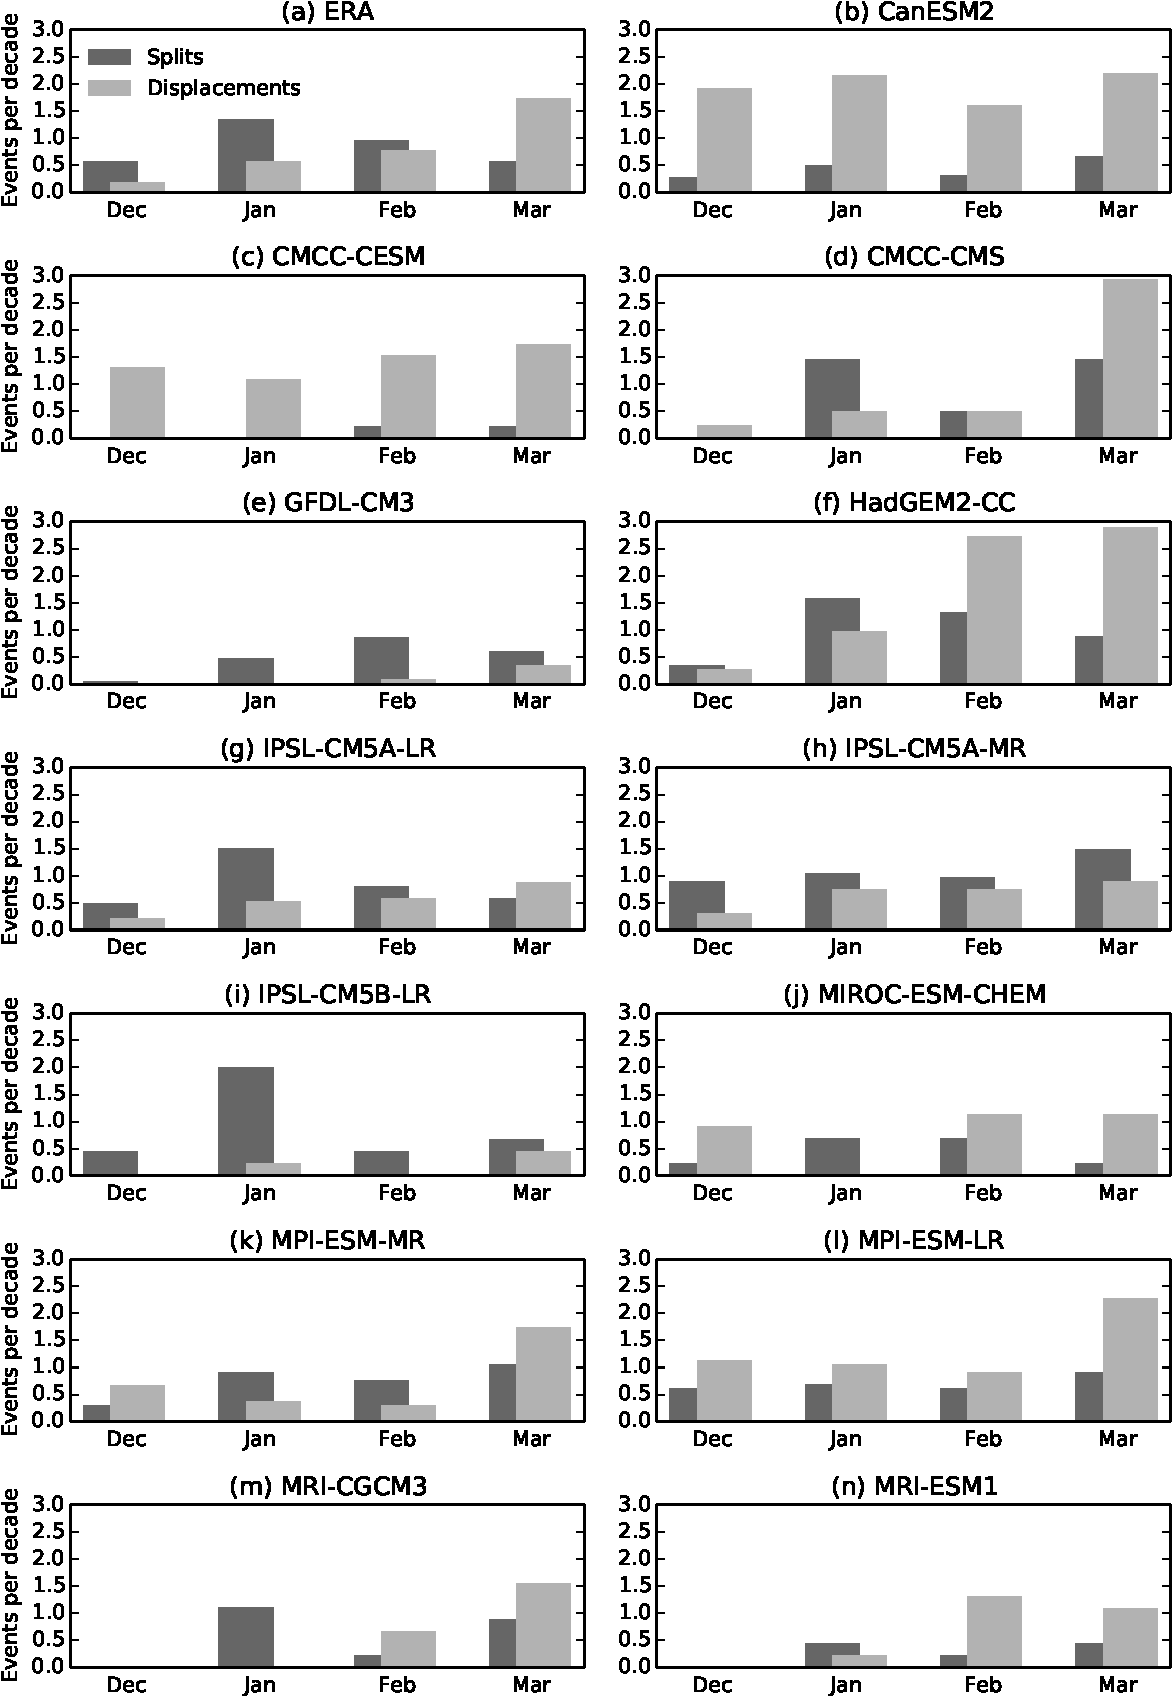
\includegraphics[width=\textwidth]{figures/chapter-models/events_seasonal.pdf}
 \caption[Seasonal distribution of splits and displacements in the CMIP5
 models]{Seasonal distribution of the occurrence of split and displaced vortex
   events in ERA (a) and the CMIP5 models.}
 \label{Fig2}
\end{figure}



\begin{figure}
 \centering
 \noindent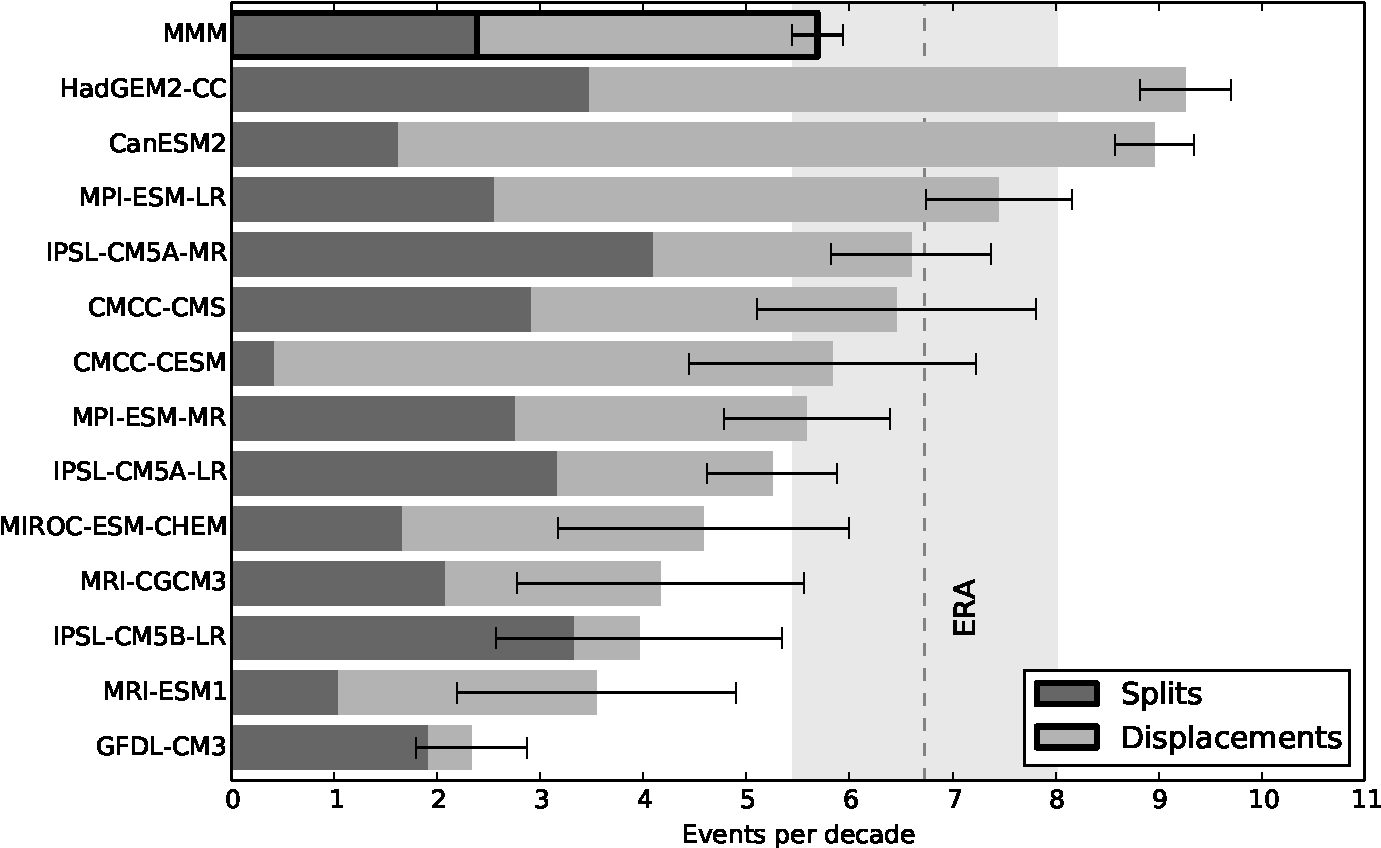
\includegraphics[width=\textwidth]{figures/chapter-models/events_bar_stacked.pdf}
 \caption[Frequency of split and displaced vortex events in the CMIP5
 models]{Frequency of split and displaced vortex events in the CMIP5
   models. Error bars are for the frequency of all events, and represent one
   $\sigma$ range, assuming a binomial distribution of events. The grey shaded
   region represents the one $\sigma$ range for ERA, along with the mean (dashed
   line.) }
 \label{Fig2}
\end{figure}

\begin{figure}
 \centering
 \noindent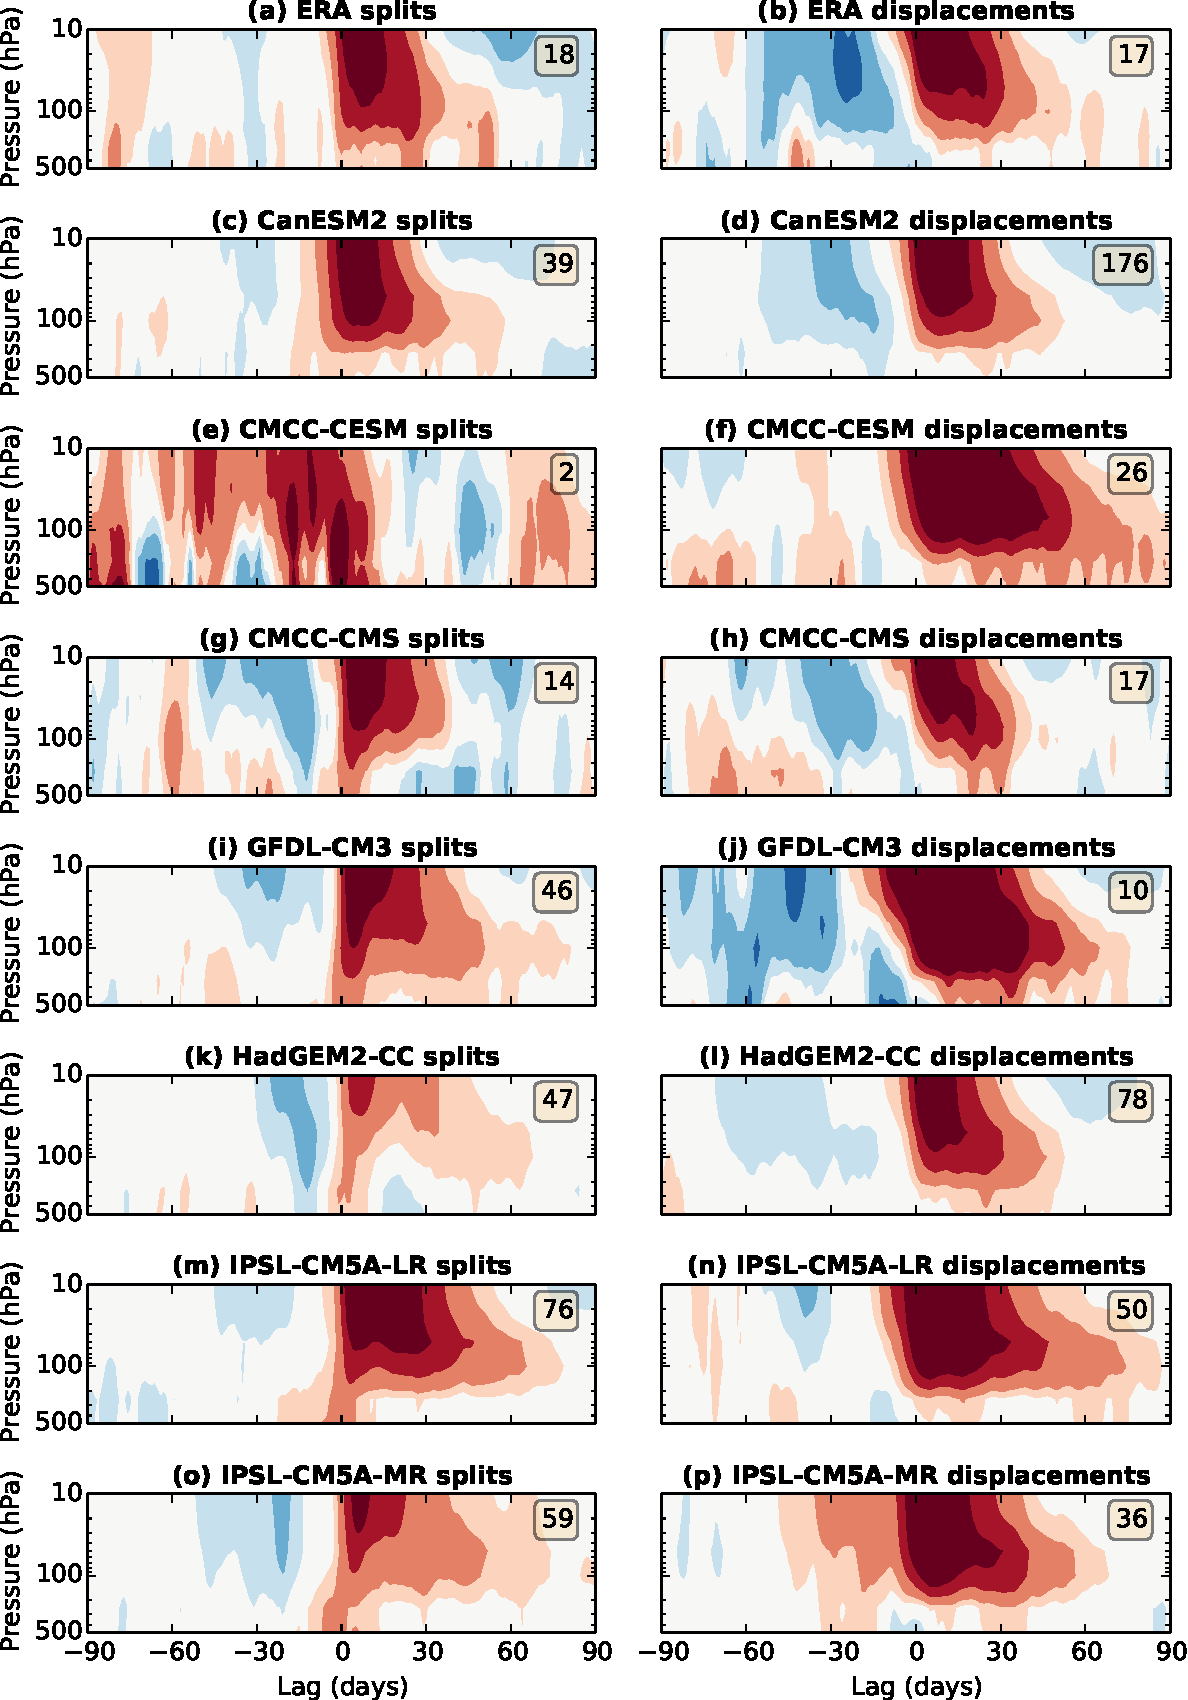
\includegraphics[width=\textwidth]{figures/chapter-models/dripping_paint1.pdf}
 \caption[NAM composites for splits and displacements in the CMIP5
 models]{Composites of normalised polar cap averaged $Z$ anomalies following
   split and displaced vortex events in ERA (a,b) and the CMIP5 models. Numbers
   in the upper right of each plot represent the number of events entering the
   composite.}
 \label{Fig2}
\end{figure}

\begin{figure}
 \ContinuedFloat
 \centering
 \noindent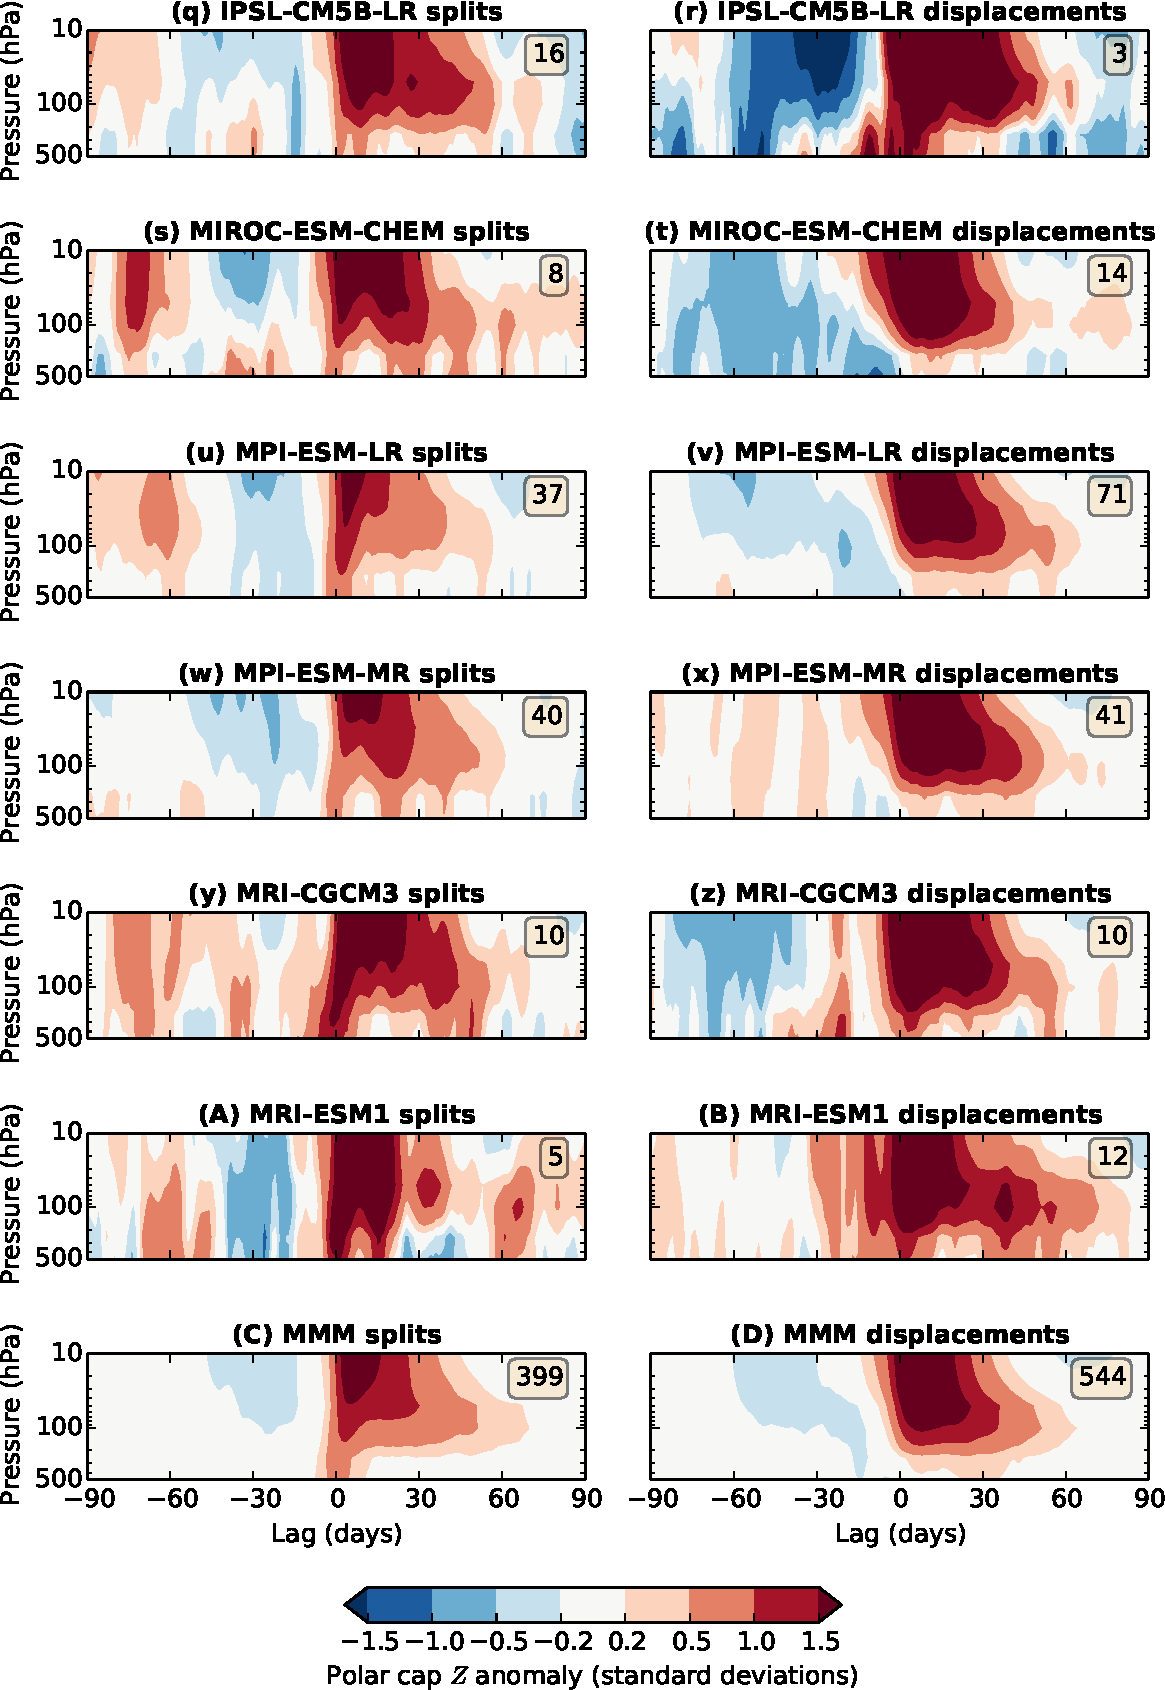
\includegraphics[width=\textwidth]{figures/chapter-models/dripping_paint2.pdf}
 \caption[]{(Continued)}
 \label{Fig2}
\end{figure}

%%% Local Variables:
%%% mode: latex
%%% TeX-master: "thesis"
%%% End:
